% SICE SI 予稿原稿．登壇者の○は第一著者に付している．
% この環境では Biber が未導入のため，BibLaTeX の BibTeX backend を使用する．
\PassOptionsToPackage{backend=bibtex}{biblatex}
\documentclass{sice-si}
\addbibresource{manuscript_references.bib}
\hypersetup{pdfauthor={Soma Okamoto and Kosuke Sekiyama}}
\newenvironment{dotsubequations}{%
  \begin{subequations}
  \renewcommand{\theequation}{\theparentequation.\arabic{equation}}%
}{\end{subequations}}

\title{MR遠隔操作における操作対象の局所適応的な位置再整合}
\name{○岡本 宗馬（名城大学），関山 浩介（名城大学）}
\etitle{Local Position Correction of MR Teleoperation Targets\\
Based on Physical Observations after Placement}
\ename{○Soma OKAMOTO (Meijo University), and Kosuke SEKIYAMA (Meijo University)}

\begin{document}
\abst{%
This paper proposes a local adaptive registration method for a virtual bottle
in mixed reality (MR) teleoperation after placement.
A prior position distribution is constructed from MR manipulation and robot
kinematics using covariance intersection.
Physical observations from YOLO/RealSense and Meta are selected or fused
according to their stability, inter-sensor consistency, and uncertainty,
and the estimated position is reflected in the target MR bottle.
Regression tests using synthetic observations confirmed all 19 tested cases,
and an MR environment test confirmed that the estimated position was reflected
in the displayed target bottle.
Quantitative evaluation using real sensors and user experiments remains future work.
}
\maketitle

\section{緒言}
複合現実（Mixed Reality: MR）を用いたロボット遠隔操作では，実環境に対応する仮想物体をユーザが操作し，その意図を実ロボットの動作へ反映する．
先行研究MASKは，操作対象の推定，可到達性を考慮した移動，運動学的な補正を統合した共有制御の枠組みである\cite{okamoto2026mask}．
一方，連続操作に伴う位置推定のドリフトなどにより，
MR表示と実環境との空間的な不整合が生じ得る．
さらに，把持中の微小な滑りや物体と環境との接触によって，
MR上のボトルと実ボトルで異なる位置関係が生じる可能性がある．
MR空間と実環境における物理拘束の不整合例を
\Fig{fig:position_mismatch}に示す．
\vspace{-12pt}
\begin{figure}[H]
    \centering
    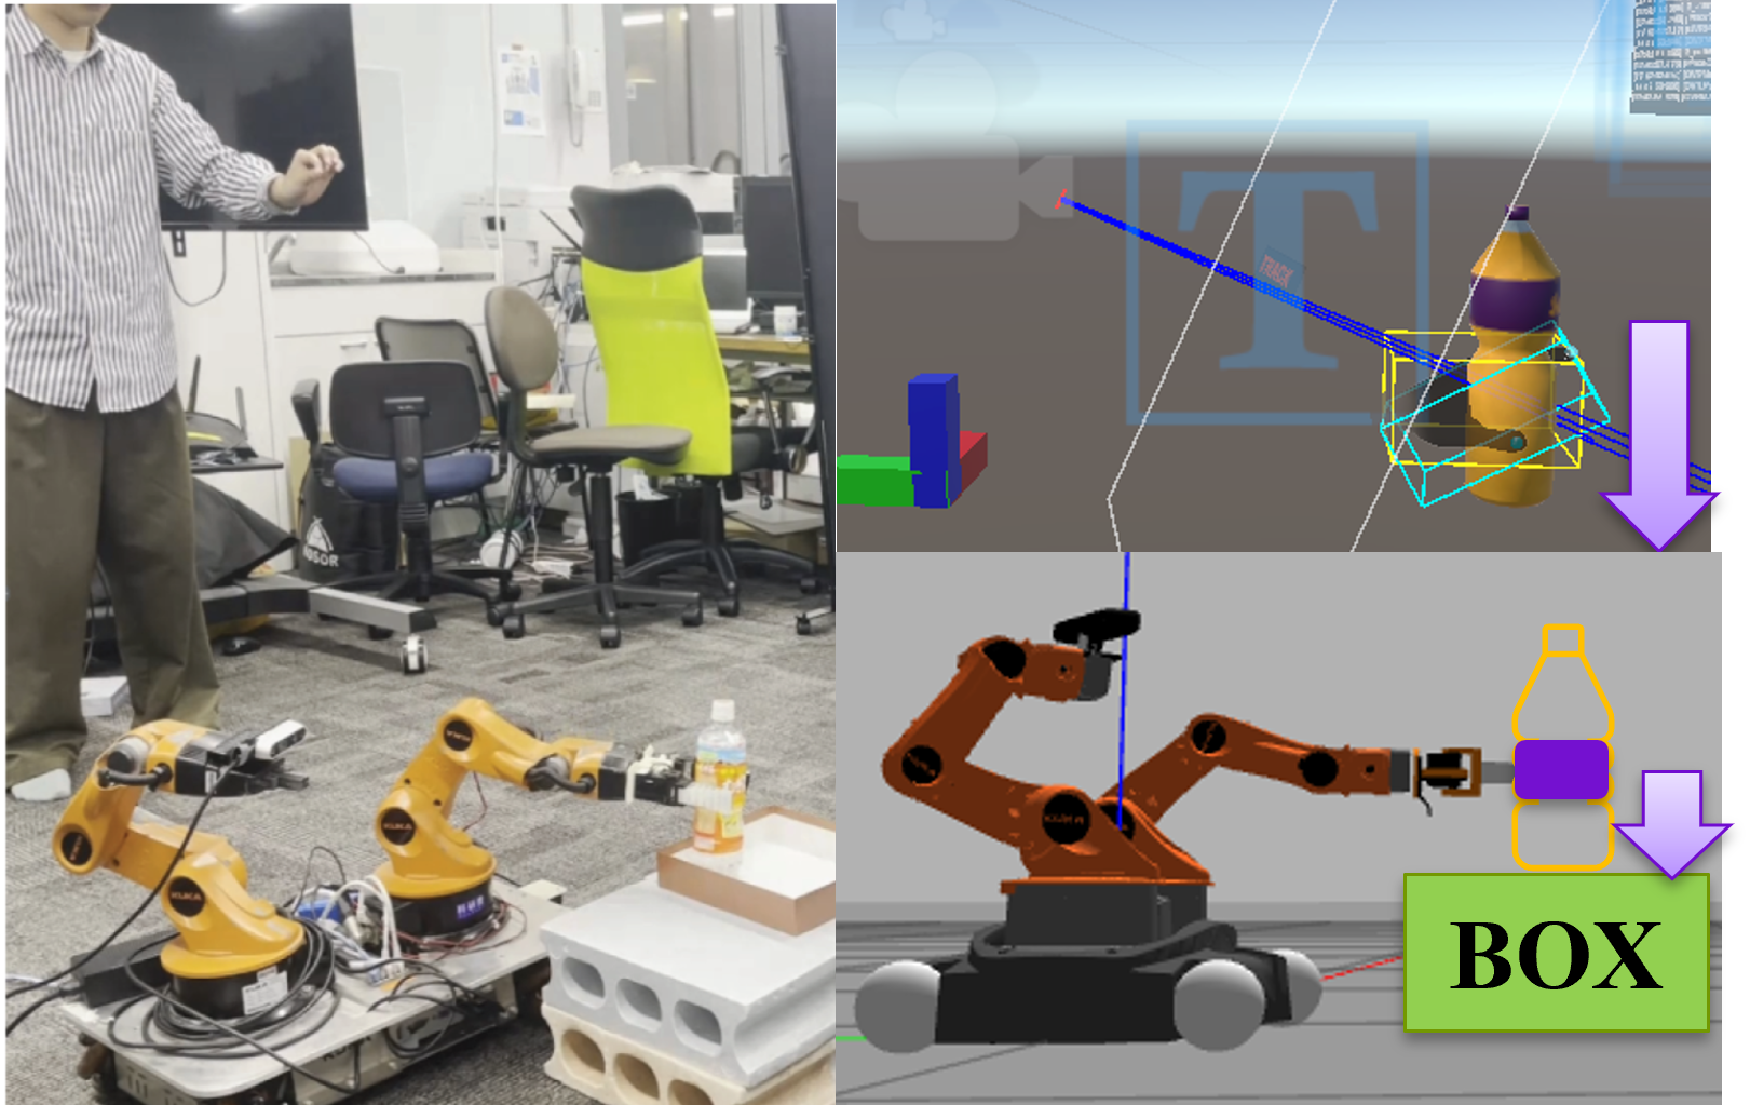
\includegraphics[width=.60\linewidth]{figures/physics1.pdf}
    \caption{Example of inconsistent physical constraints between the MR and real environments}
    \label{fig:position_mismatch}
\end{figure}
\vspace{-12pt}
そこで本研究では，Place後の物理観測を用いて対象ボトルを
局所的に再整合する手法を提案する．
MR操作と運動学情報から事前分布を構成し，
継続性と対象対応を確認した物理観測を用いてPlace後の位置を推定する．
さらに，その推定位置を対象MRボトルへ反映する．
本稿では手法を定式化するとともに，
合成データを用いた回帰テストおよびMR環境における動作確認により，
提案システムの基本動作を検証する．

\section{提案システムと事前分布}
\subsection{システム構成}

本研究では，MR遠隔操作におけるPlace後の操作対象について，
物理観測に基づいてMR上の表示位置を局所的に再整合する
局所適応レジストレーションを行う．
本手法はMR空間全体の座標変換やSLAM地図を更新するものではなく，
Place操作の対象となったボトルの並進位置のみを補正対象とする．提案する局所適応レジストレーションのシステム構成を
\Fig{fig:system_overview}に示す．
\begin{figure}[H]
    \centering
    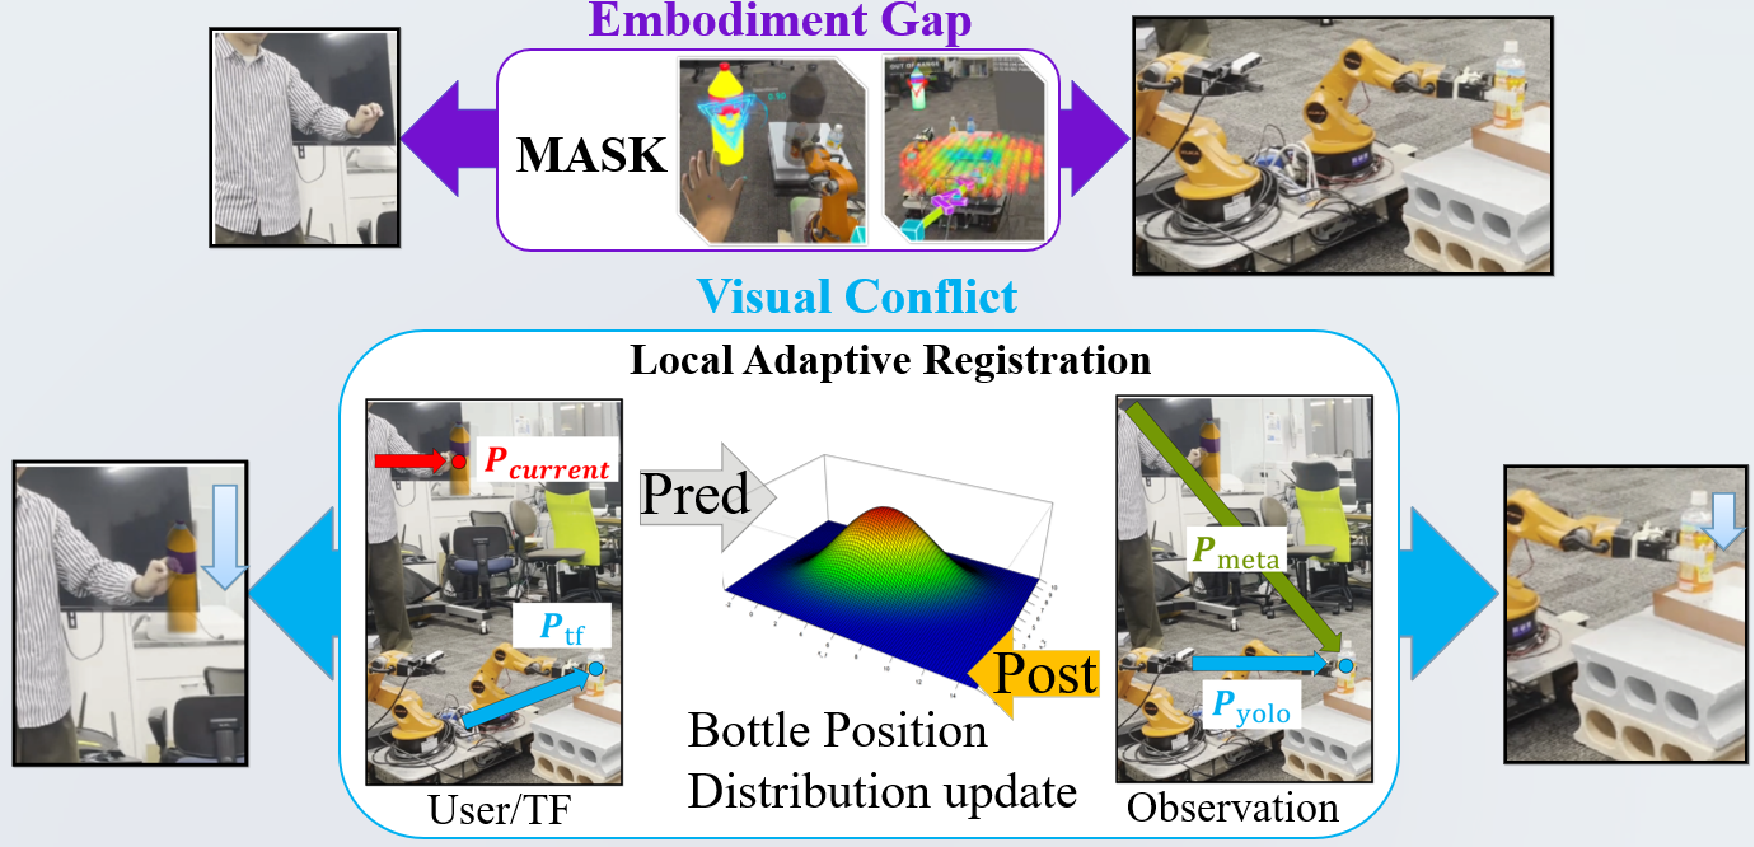
\includegraphics[width=.95\linewidth]{figures/System2.pdf}
    \caption{System overview of the local adaptive registration}
    \label{fig:system_overview}
\end{figure}
\vspace{-12pt}

まず，MR上でユーザが操作したボトル位置$P_{\mathrm{current}}$と，
ロボットのエンドエフェクタ位置に基づく$P_{\mathrm{tf}}$から，
Place後のボトル位置に対する事前分布を構成する．
次に，Place後の実ボトルをYOLO/RealSenseおよびMetaにより観測し，
複数フレームから得られる位置と共分散を用いて
観測候補の安定性とセンサ間の整合性を評価する．

事前分布の構成に用いるMR操作・ロボット運動学情報と，
Place後に用いる物理観測の概要を\Fig{fig:method_overview}に示す．
\vspace{-10pt}
\begin{figure}[H]
    \centering
    \begin{minipage}{.5\linewidth}
        \centering
        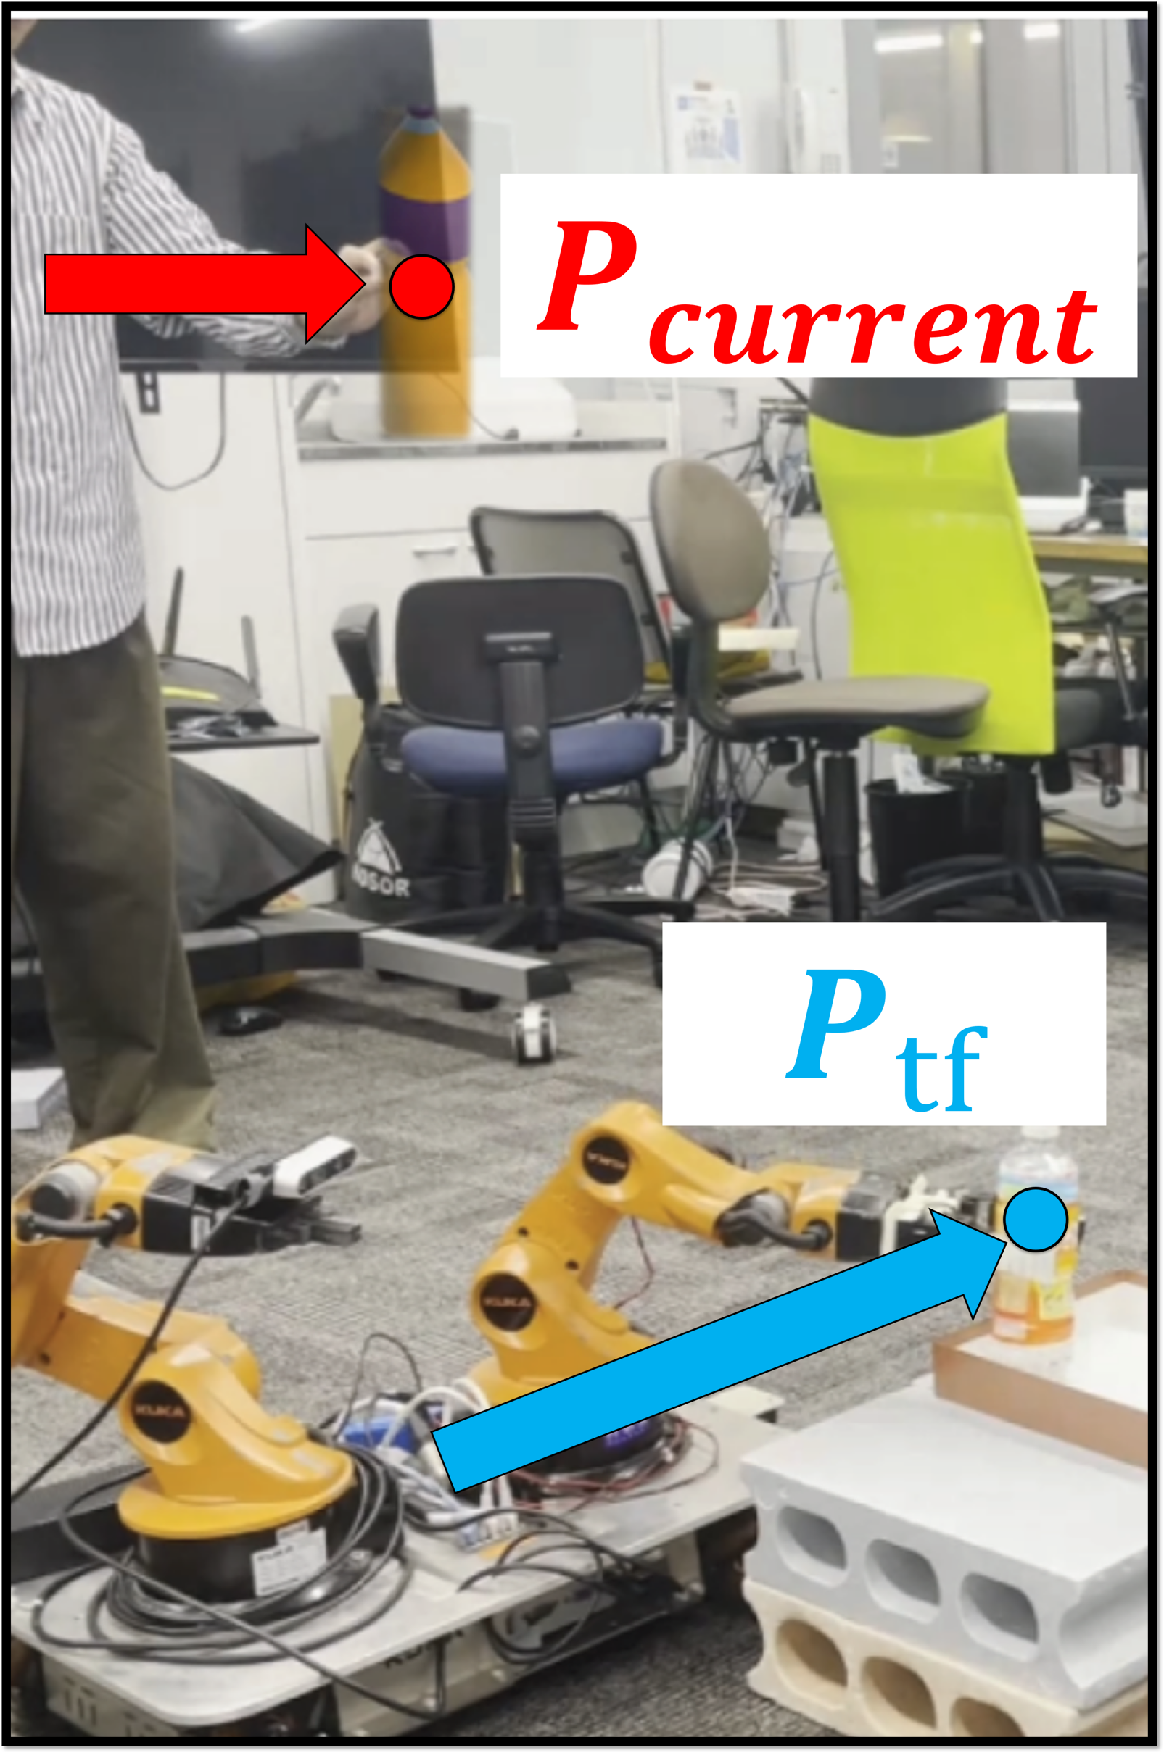
\includegraphics[width=.55\linewidth]{figures/pred_P.pdf}
        \subcaption{User and robot operation}
        \label{fig:method_prior}
    \end{minipage}%
    \begin{minipage}{.5\linewidth}
        \centering
        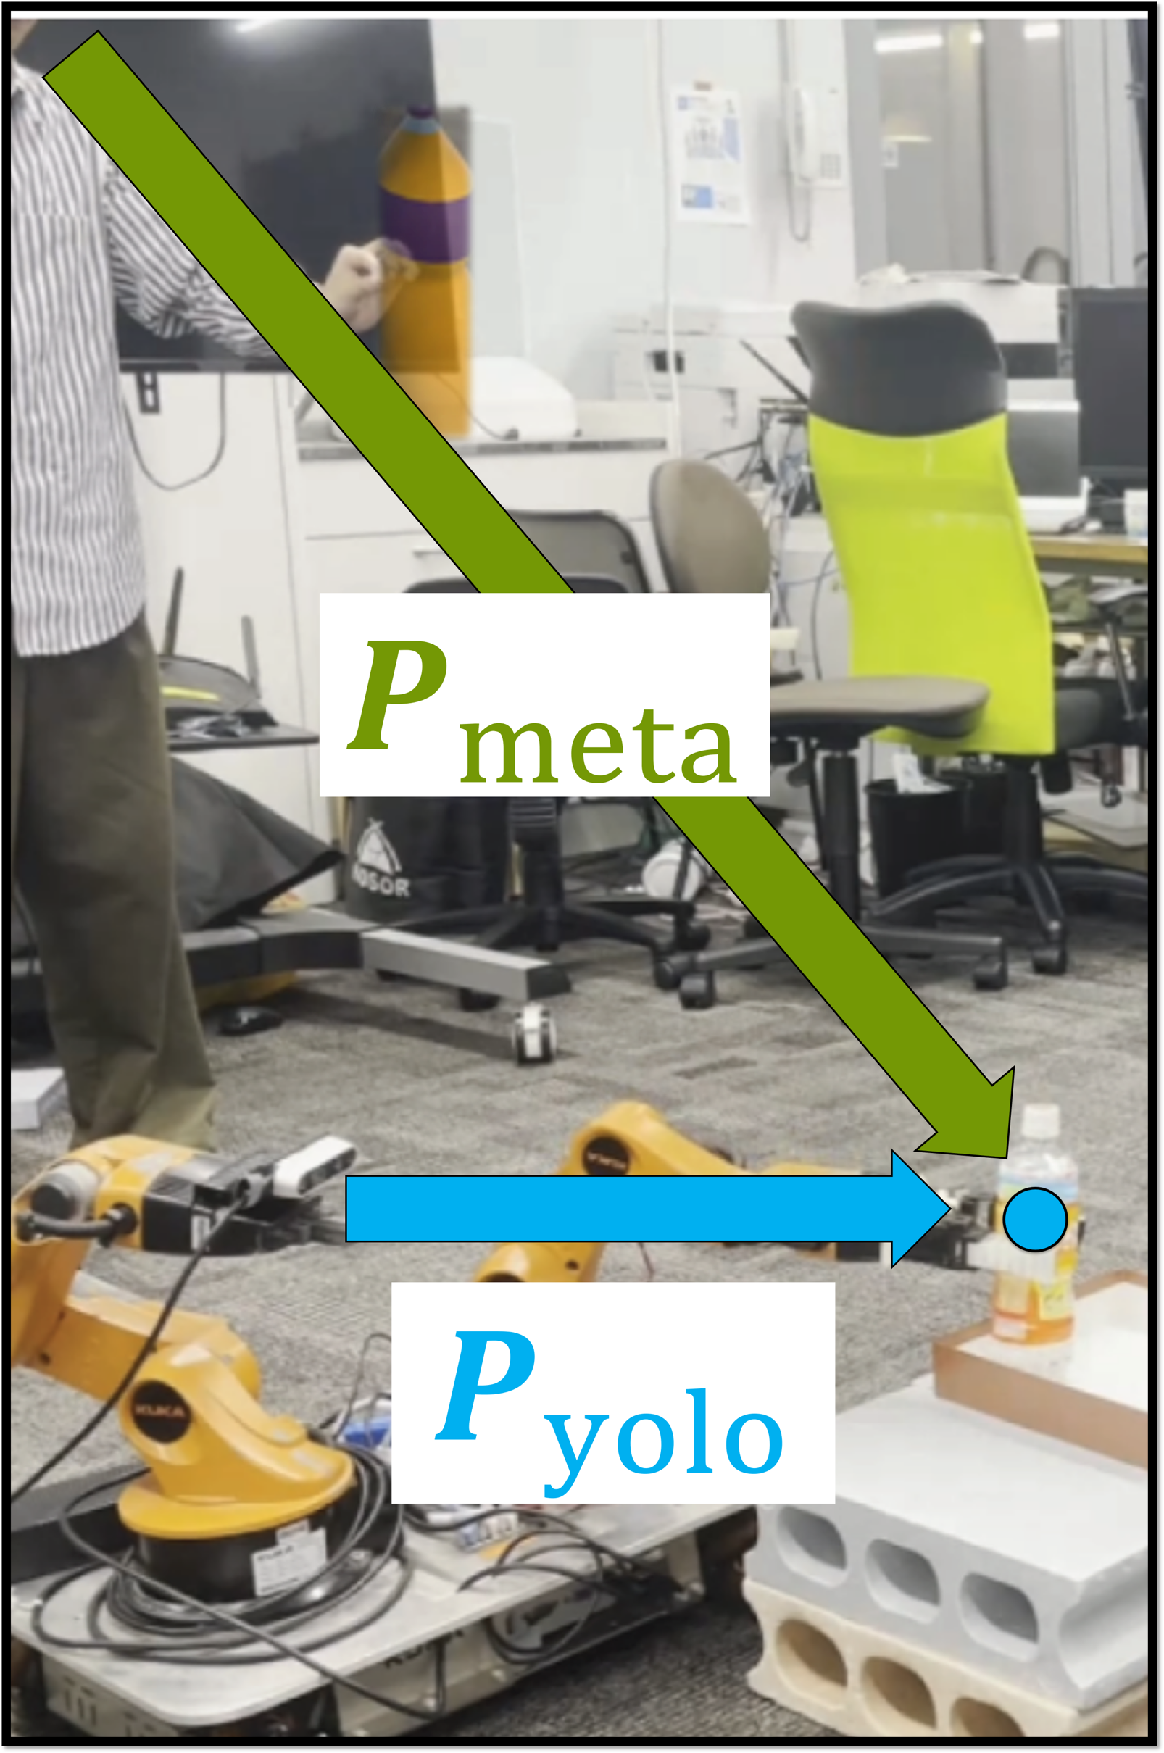
\includegraphics[width=.55\linewidth]{figures/post_P.pdf}
        \subcaption{Physical observation}
        \label{fig:method_meta}
    \end{minipage}
    \caption{Information used for local adaptive registration}
    \label{fig:method_overview}
\end{figure}
\vspace{-12pt}
有効な観測が得られた場合には，観測間の整合性と不確かさに基づいて，
観測を融合または一方を選択し，Place後の位置
$P_{\mathrm{place}}$を推定する．
一方，観測が得られない場合や，複数の観測が競合し，
不確かさからも優劣を決定できない場合には事前分布を用いる．
最後に，推定位置とMR上の現在位置との差を
操作対象ボトルの表示位置へ反映することで，
実ボトルとMRボトルの局所的な位置対応を更新する．




本稿でいう「局所」とは，補正対象をPlace操作の対象ボトルに限定し，
環境全体の座標系を変更しないことを表す．
また「適応」とは，二つの意味を含む．第一に，Place後に得られる
物理観測に応じて，事前分布と観測の利用方針を試行内で変更し，
その試行の位置推定とMR上の位置対応へ反映することを表す．
第二に，操作情報と物理観測との差から各情報源の誤差特性を
試行間で逐次更新し，次試行以降の事前分布へ反映することを表す．

\subsection{事前位置分布の構成}
推定対象をPlace後のボトル中心位置$x\in\mathbb{R}^{3}$とする．$P_{\mathrm{current}}$は，MR上のロボットオブジェクトに対する，
ユーザが操作したMRボトルの相対位置を表す．$P_{\mathrm{tf}}$は，実ロボットの\texttt{base\_link}からエンドエフェクタ（EE）への相対位置に基づく位置情報である．
両者を同じボトル中心の推定値として扱うため，座標軸・単位・基準時刻をそろえ，EE姿勢を用いて把持オフセットを変換する．以降は，共通座標系でボトル中心へ換算した位置も同じ記号で表す．
共分散もこの座標系へ変換し，把持オフセットや座標変換の不確かさを考慮する．

各操作情報$o\in\{\mathrm{current},\mathrm{tf}\}$について，
試行$t$における位置情報を
\begin{dotsubequations}
\label{eq:operation-error-model}
\begin{align}
P_o^{(t)} &= x^{(t)}+b_o+\epsilon_o^{(t)},\\
\epsilon_o^{(t)} &\sim \mathcal{N}(0,\Sigma_o),\\
\tilde P_o^{(t)}&=P_o^{(t)}-\hat b_o,\\
p(x\mid P_o^{(t)})
&=\mathcal{N}(x;\tilde P_o^{(t)},\hat\Sigma_o)
\end{align}
\end{dotsubequations}
と表す．ここで，$x^{(t)}$は試行$t$における実際のPlace位置を表す
潜在量，$b_o$は情報源$o$が持つ系統的バイアス，
$\epsilon_o^{(t)}$は試行ごとのランダム誤差，$\Sigma_o$はその共分散である．
後述する誤差特性の逐次更新では，$\hat b_o$と$\hat\Sigma_o$を更新し，
次試行以降の事前分布へ反映する構成を定義する．
学習済みバイアスを用いる場合は平均値を補正し，各情報源の分布として扱う．
本稿ではこの誤差特性更新の理論を定義し，
次試行の事前分布への反映は今後の実装・検証課題とする．

各位置情報を共分散付きのガウス分布として
\begin{dotsubequations}
\label{eq:inputs}
\begin{align}
p(x\mid P_{\mathrm{current}})
  &=\mathcal{N}(x;P_{\mathrm{current}},\Sigma_{\mathrm{current}}),\\
p(x\mid P_{\mathrm{tf}})
  &=\mathcal{N}(x;P_{\mathrm{tf}},\Sigma_{\mathrm{tf}})
\end{align}
\end{dotsubequations}
と表す．式\eqref{eq:inputs}では，必要に応じて
$P_{\mathrm{current}}$，$P_{\mathrm{tf}}$，
$\Sigma_{\mathrm{current}}$，$\Sigma_{\mathrm{tf}}$が
式\eqref{eq:operation-error-model}に基づく学習済み誤差特性を反映した量となる．
以下，逆行列を用いる共分散は正定値として扱う．

\subsection{共分散交差法による事前分布の構成}
両位置情報の誤差の相互相関は不明であるため，共分散交差法（Covariance Intersection: CI）\cite{ajgl2022ci_partial}を用いる．事前位置と共分散を
\begin{dotsubequations}
\begin{equation}
\Sigma_{\mathrm{pred}}^{-1}
 =\omega\Sigma_{\mathrm{current}}^{-1}
 +(1-\omega)\Sigma_{\mathrm{tf}}^{-1}
\label{eq:prior-cov}
\end{equation}
\vspace{-4pt}
\begin{equation}
\begin{aligned}
P_{\mathrm{pred}}
&=\Sigma_{\mathrm{pred}}\left(
\begin{aligned}
&\omega\Sigma_{\mathrm{current}}^{-1}P_{\mathrm{current}}\\
&+(1-\omega)\Sigma_{\mathrm{tf}}^{-1}P_{\mathrm{tf}}
\end{aligned}
\right)
\end{aligned}
\label{eq:prior-mean}
\end{equation}
\vspace{-4pt}
\begin{equation}
p^{-}(x)=\mathcal{N}(x;P_{\mathrm{pred}},\Sigma_{\mathrm{pred}}),
\quad 0\leq\omega\leq1
\label{eq:prior}
\end{equation}
\end{dotsubequations}
と定義する．$P_{\mathrm{current}}$はMR操作を反映するが，接触などの物理拘束を必ずしも反映しない．EEから換算した位置も，滑りや解放後の移動を直接観測したものではない．$p^{-}(x)$はPlace後の実ボトルを観測する前の予測を表す．

\section{物理観測による位置推定}
\subsection{複数フレームによる観測候補の構成}
センサ集合を$s\in\{Y,M\}$とし，$Y$をYOLO/RealSense，$M$をMetaとする．Place後にボトルが静止しているとみなせる観測区間を設け，
各センサの複数フレームから，同じ物理ボトルに対応する候補$j$を構成する．観測位置は事前分布と同じ座標系のボトル中心へ換算する．

画像認識とPointCloudを組み合わせて観測を構成する．YOLO/RealSenseはRGB-Dカメラであり，RGB画像から物体検出を行い，深度画像から三次元位置を求める．
MetaはRGBカメラとステレオカメラを備え，視差から三次元位置を求める．
MetaからのPointCloudはデータ数が多いため，チャンク分割後にタスク範囲へ限定して処理する．

ここではセンサ添字$s$を省略する．候補$j$の三次元位置$z_{j,n}$とフレーム数$N_j\geq2$から，代表位置$\bar z_j$，フレーム間の標本共分散$C_{\mathrm{frame},j}$，
代表位置の観測共分散$R_{\mathrm{frame},j}$を
\begin{dotsubequations}
\begin{align}
\bar z_j=\frac{1}{N_j}\sum_{n=1}^{N_j}z_{j,n},
\label{eq:mean}\\
C_{\mathrm{frame},j}=\frac{1}{N_j-1}\sum_{n=1}^{N_j}
(z_{j,n}-\bar z_j)(z_{j,n}-\bar z_j)^{\mathsf T},
\label{eq:sample-cov}\\
R_{\mathrm{frame},j}=\frac{C_{\mathrm{frame},j}}{N_j}
\label{eq:mean-cov}
\end{align}
\end{dotsubequations}
により求める．式\eqref{eq:mean-cov}はフレームごとの誤差が独立な場合の代表位置の不確かさを表す．
時間相関や共通の座標変換誤差がある場合，$1/N_j$倍では過小評価し得るため，それらを観測共分散に考慮する．フレーム間のばらつきの小ささは，系統誤差の小ささを保証しない．

以降，代表位置を$z_{s,j}$，その観測共分散を$R_{s,j}$と表す．
各センサ$s\in\{Y,M\}$の代表観測は
\begin{dotsubequations}
\label{eq:observation-model}
\begin{align}
z_{s,j}^{(t)} &= x^{(t)}+v_{s,j}^{(t)},\\
v_{s,j}^{(t)} &\sim \mathcal{N}(0,R_{s,j}^{(t)})
\end{align}
\end{dotsubequations}
に従うと仮定する．ここで観測誤差$v_{s,j}^{(t)}$は零平均とする．
この仮定は，後述する操作情報側の系統的バイアス$b_o$の推定に用いる．
検出の継続性と位置のばらつきから安定性を判定し，対象対応と共分散評価を確認した安定な候補を有効観測とする．
不安定，未検出，対象対応または共分散評価が不確かな候補は無効とする．
また，観測共分散$R_{s,j}$の最大固有値から求めた
最大主軸標準偏差$\sqrt{\lambda_{\max}(R_{s,j})}$に上限
$\sigma_{\max}$を設け，上限を超える候補は無効とする．

\subsection{事前予測および観測間の整合度}
事前予測と各候補との不整合を，マハラノビス距離\cite{orou_mousse2023localization_uncertainty}の二乗$d^{2}_{s,j}$と整合度$l_{s,j}$により
\begin{dotsubequations}
\label{eq:prior-consistency}
\begin{align}
v_{s,j}&=z_{s,j}-P_{\mathrm{pred}},\\
S_{s,j}&=\Sigma_{\mathrm{pred}}+R_{s,j},\\
d^{2}_{s,j}&=v_{s,j}^{\mathsf T}S_{s,j}^{-1}v_{s,j},\\
l_{s,j}&=\exp(-d^{2}_{s,j}/2)
\end{align}
\end{dotsubequations}
で表す．これらは予測と観測の整合度を示す指標であり，観測の正誤を単独では決めない．事前予測自体の位置ずれを補正するため，$P_{\mathrm{pred}}$から離れていても，
同じ物理ボトルの安定した有効観測は位置推定に利用する．
すなわち，事前分布$p^{-}(x)$は物理世界の完全な予測ではない．
特に$P_{\mathrm{current}}$はMR空間上でユーザが操作した仮想物体位置を含むため，
物理観測が$P_{\mathrm{pred}}$から離れていることだけを理由に誤観測とは判断しない．
むしろMR側の事前予測自体が物理世界からずれている可能性があるため，
信頼できる物理観測は位置推定に用いる．

YOLO/RealSenseとMetaの双方に有効な候補がある場合，選択された位置$P_{\mathrm{yolo}}$，$P_{\mathrm{meta}}$と対応する共分散$R_{\mathrm{yolo}}$，$R_{\mathrm{meta}}$を用いて
\begin{dotsubequations}
\label{eq:sensor-consistency}
\begin{align}
e_{YM}&=P_{\mathrm{yolo}}-P_{\mathrm{meta}},\\
S_{YM}&=R_{\mathrm{yolo}}+R_{\mathrm{meta}},\\
d^{2}_{YM}&=e_{YM}^{\mathsf T}S_{YM}^{-1}e_{YM}
\end{align}
\end{dotsubequations}
を計算する．同一対象についての両観測の整合性を閾値$\tau_{YM}$で判定する．この閾値は観測間距離のみに用い，事前予測との距離には適用しない．
共分散の大小は各軸の分散の合計$\operatorname{tr}(R_s)$で比較する．
観測同士が競合する場合には，$\operatorname{tr}(R_s)$が小さい観測を採用する．
一方，両観測の不確かさが同程度で優劣を決定できない場合には，
いずれの観測も採用せず，事前分布へフォールバックする．
この「同程度」を判定する具体的な閾値は，今後設定する．

式\eqref{eq:prior-consistency}と式\eqref{eq:sensor-consistency}は相互相関を含まない近似であり，厳密な確率検定として解釈しない．
$l_{s,j}$も正規化された尤度や観測の正答確率ではなく，整合度の指標である．

\subsection{観測後の位置推定分布}
利用可能な観測集合を$\mathcal{A}\subseteq\{Y,M\}$とし，$P_Y=P_{\mathrm{yolo}}$，$P_M=P_{\mathrm{meta}}$とする．共分散$R_Y$，$R_M$も同様に対応させる．
事前予測および観測間の誤差相関が不明であることを考慮し，
観測後の位置と共分散をCIにより更新する．
事前予測と有効観測が近い場合には，事前分布を補助情報として
\begin{dotsubequations}
\begin{align}
\Sigma_{\mathrm{place}}=
\left(\omega_0\Sigma_{\mathrm{pred}}^{-1}
+\sum_{s\in\mathcal{A}}\omega_s R_s^{-1}\right)^{-1},
\label{eq:place-cov}\\
P_{\mathrm{place}}=\Sigma_{\mathrm{place}}
\left(\omega_0\Sigma_{\mathrm{pred}}^{-1}P_{\mathrm{pred}}
+\sum_{s\in\mathcal{A}}\omega_s R_s^{-1}P_s\right),
\label{eq:place-mean}\\
\omega_0+\sum_{s\in\mathcal{A}}\omega_s=1,
\qquad \omega_0,\omega_s\geq0
\label{eq:weights}
\end{align}
\end{dotsubequations}
と融合する．これに対し，事前予測と有効観測が遠い場合には，
MR側の事前予測自体が物理世界からずれている可能性を考慮し，
$\omega_0=0$として物理観測のみで
\begin{dotsubequations}
\begin{align}
\Sigma_{\mathrm{place}}=
\left(\sum_{s\in\mathcal{A}}\omega_s R_s^{-1}\right)^{-1},
\label{eq:place-cov-obs}\\
P_{\mathrm{place}}=\Sigma_{\mathrm{place}}
\left(\sum_{s\in\mathcal{A}}\omega_s R_s^{-1}P_s\right)
\label{eq:place-mean-obs}
\end{align}
\end{dotsubequations}
と更新する．事前予測と観測が近いか遠いかは，
式\eqref{eq:prior-consistency}の$d^2_{s,j}$を用いて判定する．
信頼できる物理観測が存在しない場合は
$P_{\mathrm{place}}=P_{\mathrm{pred}}$，
$\Sigma_{\mathrm{place}}=\Sigma_{\mathrm{pred}}$として事前分布を採用する．
これにより，観測後の位置推定分布は
\begin{equation}
p^{+}(x)=\mathcal{N}(x;P_{\mathrm{place}},\Sigma_{\mathrm{place}})
\label{eq:posterior}
\end{equation}
となる．これはCIにより構成した推定分布であり，独立な尤度の積による厳密なベイズ事後分布を意味しない．
理論上，CI重みは融合後共分散のtraceを小さくするように決定する．

対象対応と共分散評価の確認を前提に，以下の規則で観測を選択する．
\begin{enumerate}[label=(\arabic*), leftmargin=*, nosep]
\item 両方が安定し，観測同士が近い場合
（$d^{2}_{YM}\leq\tau_{YM}$）：
$\mathcal{A}=\{Y,M\}$としてCIで融合する．
さらに事前予測と観測が近い場合は式\eqref{eq:place-cov}，
式\eqref{eq:place-mean}を用い，遠い場合は式\eqref{eq:place-cov-obs}，
式\eqref{eq:place-mean-obs}を用いる．

\item 両方が安定し，観測同士が遠く
（$d^{2}_{YM}>\tau_{YM}$），
かつ不確かさに差がある場合：
$\operatorname{tr}(R_s)$が小さい一方を採用し，
事前予測との距離に応じて事前分布との融合または観測のみの更新を行う．

\item 両方が安定しているが，観測同士が遠く，
不確かさからも優劣を決定できない場合：
$\mathcal{A}=\varnothing$，$\omega_0=1$として事前分布を採用する．

\item 片方だけが安定している場合：
その有効観測のみを採用し，事前予測との距離に応じて
事前分布との融合または観測のみの更新を行う．

\item 有効な観測が存在しない場合：
$\mathcal{A}=\varnothing$，$\omega_0=1$として事前分布を採用する．
\end{enumerate}

\Fig{fig:prior_posterior}に，そのときのGazebo上のロボットモデルと，
RViz（TF）上に表示した三次元共分散楕円体を示す．
青色の楕円体は事前共分散，赤色の楕円体は観測後共分散を表す．

\vspace{2pt}
\noindent\begin{minipage}{\linewidth}
    \captionsetup{type=figure}
    \centering
    \begin{minipage}{.5\linewidth}
        \centering
        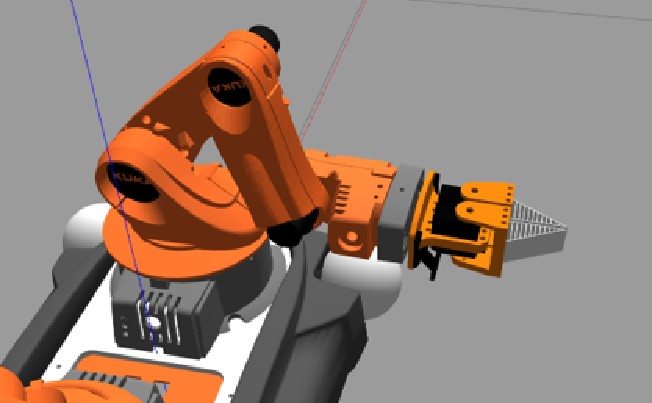
\includegraphics[width=.9\linewidth]{figures/Prior_Post_gazebo.pdf}
        \subcaption{Robot model in Gazebo}
        \label{fig:prior_post_gazebo}
    \end{minipage}%
    \begin{minipage}{.5\linewidth}
        \centering
        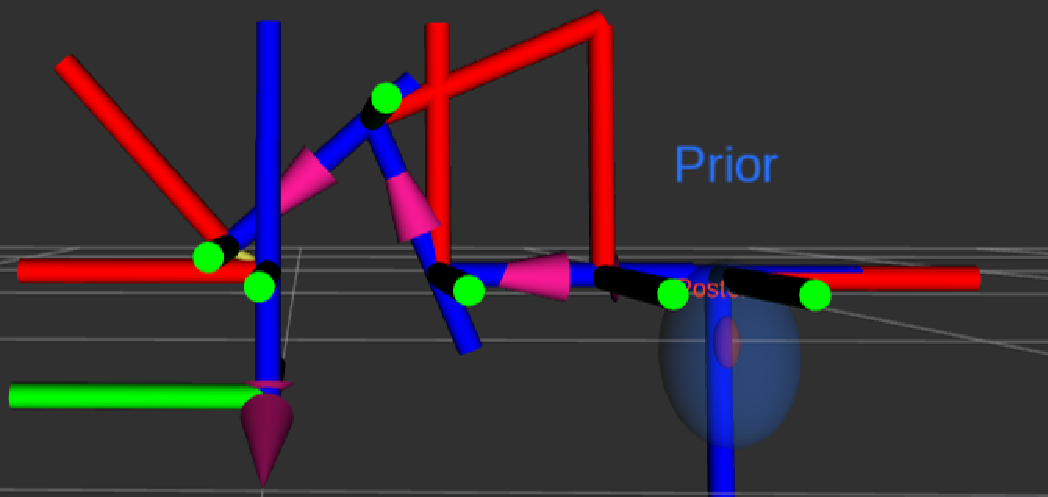
\includegraphics[width=.9\linewidth]{figures/Prior_Post_Rviz.pdf}
        \subcaption{Covariance ellipsoids in RViz}
        \label{fig:prior_post_rviz}
    \end{minipage}
    \caption{Robot model in Gazebo and prior/post-observation covariance ellipsoids in RViz/TF}
    \label{fig:prior_posterior}
\end{minipage}
\vspace{0pt}

未検出などで観測が無効な場合も同じ規則を適用する．
一方のみの採用では
$P_{\mathrm{place}}=P_s$，
$\Sigma_{\mathrm{place}}=R_s$となる．
有効観測が存在しない場合，または観測が競合し
不確かさから優劣を決定できない場合には，
$P_{\mathrm{place}}=P_{\mathrm{pred}}$，
$\Sigma_{\mathrm{place}}=\Sigma_{\mathrm{pred}}$となる．
\vspace{2pt}

\section{MRボトル補正と誤差特性更新}
\subsection{MRボトルの局所補正}
$P_{\mathrm{place}}$と$P_{\mathrm{current}}$を，同一座標系のボトル中心位置として表した上で，補正量と補正後の位置を
\begin{dotsubequations}
\begin{align}
\Delta P&=P_{\mathrm{place}}-P_{\mathrm{current}},
\label{eq:delta}\\
P_{\mathrm{registered}}&=P_{\mathrm{current}}+\lambda\Delta P,
\quad 0\leq\lambda\leq1
\label{eq:registration}
\end{align}
\end{dotsubequations}
とする．$\lambda$は推定位置をMR表示へ反映する割合を表し，$\lambda=1$では推定位置へ一致させ，$\lambda=0$では表示位置を維持する．$0<\lambda<1$では位置差の一部を反映する．
補正後の中心位置をMR表示座標へ変換し，Place操作の対象ボトルに適用することで，観測された実ボトル位置へ局所的に再整合する．補正対象は当該ボトルの並進位置であり，姿勢や他の物体，SLAM地図全体は変更しない．

\subsection{誤差特性の逐次更新}
試行$t$で実際に位置推定に使用した物理観測を
$q_{\mathrm{used}}^{(t)}(x)=\mathcal{N}(x;\bar z_{\mathrm{used}}^{(t)},R_{\mathrm{used}}^{(t)})$
とする．各操作情報$o\in\{\mathrm{current},\mathrm{tf}\}$について，操作情報と使用観測との差から
\begin{dotsubequations}
\begin{align}
e_o^{(t)}&=P_o^{(t)}-\bar z_{\mathrm{used}}^{(t)},\\
e_o^{(t)}&=b_o+\epsilon_o^{(t)}-v_{\mathrm{used}}^{(t)},\\
\hat b_o^{(n)}
&=\hat b_o^{(n-1)}
+\frac{1}{n}\left(e_o^{(n)}-\hat b_o^{(n-1)}\right)
\label{eq:bias-update}
\end{align}
\end{dotsubequations}
として系統的バイアスを逐次更新する．さらに，$r_o^{(t)}=e_o^{(t)}-\hat b_o$とし，操作情報と物理観測との差には両方のランダム誤差が含まれることから，
\begin{dotsubequations}
\begin{align}
C_o&=\frac{1}{n-1}\sum_{t=1}^{n}r_o^{(t)}r_o^{(t)\mathsf T},\\
\overline R_{\mathrm{used}}&=\frac{1}{n}\sum_{t=1}^{n}R_{\mathrm{used}}^{(t)},\\
\hat\Sigma_o&=C_o-\overline R_{\mathrm{used}}
\label{eq:cov-update}
\end{align}
\end{dotsubequations}
によりランダム誤差共分散を推定する．数値誤差により負の固有値が生じる場合は，共分散行列の対称化や最小分散の確保により正定値または半正定値性を保つ．更新した$\hat b_o$および$\hat\Sigma_o$は，式\eqref{eq:operation-error-model}を通じて次試行の事前分布へ反映する．適応の進行は，今後，事前分布と観測後分布の差をKL情報量などで評価する．ただし，独立な真値位置を直接測定していないため，真値に対する位置推定精度の向上は直接結論しない．

\vspace{4pt}
\section{実験・結果}

\subsection{検証方法}
観測融合ノードの基本動作を確認するため，合成した三次元位置および共分散を入力する回帰テストを実施した．
観測候補の選別，センサ間の整合・競合，観測欠損，不正な共分散，入力形式への対応を検証した．
テストは19メソッドで構成した．

代表条件のうち，共分散上限制約の確認では
$\sigma_{\max}=0.10$ mとした．
また，両観測を融合する整合条件では，
CIの重みを$\omega_Y=\omega_M=0.5$とした．
理論上は融合後共分散のtraceを最小化するCI重みを用いるが，
本回帰テストでは分岐動作の確認を目的として重みを固定した．

また，MR環境で推定結果が操作対象ボトルの表示位置更新へ反映されることを確認した．
代表条件として，$P_Y=[0,0,0]$ m，$P_M=[0.01,0,0]$ mの近接する2観測では中間位置を出力し，1 m離れた競合観測では不確かさの小さい0.02 m側を採用した．
一方，双方が$\sigma=0.02$ mで競合する場合，有効観測が存在しない場合には事前分布へフォールバックし，最大主軸標準偏差が上限0.10 mを超える候補は棄却した．

\subsection{結果}
回帰テストは19件中19件が成功し，失敗，エラー，スキップはいずれも0件であった．
観測が整合する条件では両観測の中間位置が得られ，観測が競合し不確かさが異なる条件では，共分散の小さい観測が採用された．
一方，観測が競合し不確かさを区別できない条件および有効な観測が存在しない条件では，事前分布へフォールバックすることを確認した．
また，設定した最大主軸標準偏差の上限を超える観測候補が棄却されることを確認した．
以上より，観測の採用，棄却，融合，およびMR表示への反映に関する一連の分岐が想定通り動作することを確認した．

\vspace{4pt}
\section{結言}
本稿では，Place後の物理観測に基づいて操作対象ボトルのMR表示位置を局所的に再整合する手法を提案した．MR操作情報とロボット運動学情報から事前分布を構成し，YOLO/RealSenseおよびMetaによる物理観測を安定性，整合性，不確かさに基づいて選択・融合することで，Place後の対象位置を推定する構成を示した．
合成データを用いた回帰テストでは19件中19件が成功し，観測の融合，競合時の選択，事前分布へのフォールバック，不確かな観測の棄却が行われることを確認した．また，MR環境において，推定結果が操作対象ボトルの表示位置へ反映される基本動作を確認した．
本検証は合成データを中心とした基本動作の確認であり，実センサおよび実機環境における位置精度や，ユーザ操作への影響を定量的に評価したものではない．
今後は，独立な基準位置に対する補正前後の位置誤差，観測共分散および整合性判定の妥当性，CI重みと反映率$\lambda$の設定，誤差特性の逐次学習，KL情報量による適応評価を検討するとともに，実環境での定量評価およびユーザテストを行う．

\vspace{4pt}
\printbibliography[title=参考文献]
\end{document}
